\documentclass{ltjsarticle}

\usepackage{luatexja}
\usepackage{graphicx}
\usepackage[colorlinks=true,linkcolor=blue,citecolor=blue,urlcolor=blue]{hyperref}
\usepackage{xcolor}
\usepackage{mathtools}
\usepackage{siunitx}
\usepackage{amsmath}
\usepackage{amssymb}
\usepackage{sepnum} % sepnumパッケージを読み込む
\usepackage{at}
\usepackage{bm}
\usepackage{titlesec}
\numberwithin{equation}{section} % 数式番号をセクションごとに分ける
\titleformat{\subsubsection}
  {\normalfont\large\bfseries}
  {\thesubsubsection}{1em}{}



\usepackage[most]{tcolorbox}
\newtcolorbox{eqbox}[1]{%
  enhanced,
  colback=white, colframe=black,
  boxrule=0.4pt, arc=6pt,
  left=8pt, right=8pt, top=8pt, bottom=8pt, % 余白
  title={#1},                 % ← 引数がタイトルになる
  fonttitle=\bfseries,        % タイトルの体裁
  coltitle=black,
  colbacktitle=gray!10,       % タイトル帯の背景色(要らなければ white)
  attach boxed title to top left={yshift=-2mm, xshift=6pt}, % 箱内の左上に配置
  boxed title style={sharp corners, boxrule=0pt}, % タイトル枠線なし
}


\title{Introduction to Plasma Physics}
\author{中 陽太}
\date{2025年8月29日}

\begin{document}

\maketitle

% 目次
\tableofcontents

\section*{前書き}
 以下の内容は、主に

\cite{a} Francis F. Chen, "Introduction to Plasma Physics and Controlled Fusion"\par
\cite{b} 宮本健郎 『プラズマ物理の基礎』\par
\cite{c} EMANの物理学\\
を参照している。





\section{プラズマとは}
\subsection{自然界でのプラズマ}
 物質の温度を上げていくと、固体、液体、気体と相変化し、さらに温度を上げると、気体分子は原子から電子が剥ぎ取られ、プラスの電荷を持ったイオンと負の電荷を持った電子とが混じった気体になる。このような高温の電離ガス状態を\textcolor{red}{プラズマ}という。
固体、液体、気体と並んで、「第四の状態」と呼ばれることもある。

 一般的に、プラズマは真空中にしか存在しない。なぜなら、空気がプラズマを冷やし、イオンと電子を再び結合させるからである。自然界においては、宇宙空間は密度がかなり低いが一種のプラズマだし、
点灯中の蛍光灯の中やロウソクの炎などは全ての原子から電子が剥がれるほどではないがこれも一種のプラズマだし、さらにオーロラや電離層もプラズマだし、冬場に体験する静電気の放電や、溶接工事に使う電気放電、落雷などもプラズマである。太陽もまたプラズマの塊である。実に、この宇宙の99\%以上の場所がプラズマであって、地球のようなそうでない場所の方が珍しいくらいである。

 Saha方程式では、熱平衡状態にある気体において、イオン化の割合を教えてくれる。

\begin{eqbox}{Saha方程式}
\begin{equation}
\frac{n_i}{n_n} \approx 2.4 \times 10^{21} \frac{T^{3/2}}{n_i} e^{-U_i/KT} 
\end{equation}  
\end{eqbox}

ここで$n_i$はイオン化された原子の密度$[m^{-3}]$、$n_n$は原子の密度であり、$K$はボルツマン定数、$U_i$は気体のイオン化エネルギーである。

(1.1)式から、$T$が大きくなるにつれて$n_i$の割合が増える、つまり気体がプラズマ状態になることがいえる。これがプラズマが高温でのみ存在する理由である。

Saha方程式の物理的な意味を指摘すると、気体中の原子は熱エネルギーに分布があり、たまたま十分大きいエネルギーの衝突を受けると電子が飛び出して電離する。低温ではそのような“速い原子”は少なく、電離はまれ。Saha式の 
$\exp{(-U_i/KT)}$は「速い原子の数が温度に対して指数関数的に減る(=低温で急減)」ことを表す。また、いったん電離しても、電子と出会えば再結合して中性に戻る。つまり、再結合率は電子密度に依存する。これが$n_i ^{-1}$となる要因である。星間ガスでは 
$n_i \sim 1 cm^{-3}$と非常に低密度のため、再結合が遅く、高温でなくてもプラズマ状態が保たれやすい。


\subsection{プラズマの定義}
いかなるイオン化した気体をプラズマと呼ぶわけではない。プラズマの定義は次のように表される。
\begin{center}
プラズマとは、荷電粒子と中性粒子からなる準中性ガスであり、集団運動を示すものである。  
\end{center}

準中性ガスの説明は1.4節で説明する。集団運動について、これはプラズマ粒子間に働くクーロン力が遠距離まで作用することに起因している。クーロン力は$1/r^2$で減衰するのに対し、プラズマの場合、立体角を考慮すると、Aに対するBの体積は$r^3$に比例する。
そのため、遠距離においてもプラズマは影響し合っている。つまり、集団運動とは、局所的な条件だけでなく、遠隔領域におけるプラズマの状態にも依存する運動を指す。実際、これらの性質がプラズマ物理学という研究分野を豊かにしている。

\begin{figure}[htbp]
  \centering
  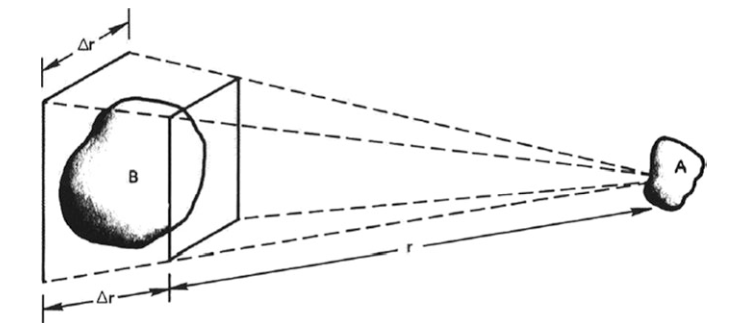
\includegraphics[width=0.7\linewidth]{solid_angle.png}
  \caption{遠距離に作用するクーロン力}
  \label{fig:sample}
\end{figure}


\subsection{温度の概念}
先に進む前に、温度の物理的な概念を見直そう。熱平衡状態の気体の速度分布はマクスウェル分布に従う。

\begin{eqbox}{一次元のマクスウェル分布}
\begin{equation}
f(u) = A \exp\left(-\frac{1}{2}mu^2/KT\right),\hspace{2pc} A = n\left(\frac{m}{2\pi KT}\right)^{1/2} \label{Max}
\end{equation}
\end{eqbox}

マクスウェル分布の導出は\url{https://www1.doshisha.ac.jp/~bukka/lecture/statistic/pdftext/std-02.pdf}を参照してほしい。

分布の幅は定数Tによって特徴づけられ、これを温度と呼ぶ。Tの正確な意味を理解するために、この分布における粒子の平均運動エネルギーを計算しよう。

\begin{equation}
 E_{av} = \frac{\int_{-\infty}^{\infty} \frac{1}{2}mu^2 f(u)du}{\int_{-\infty}^{\infty} f(u)du} \label{AV.K}
\end{equation}
ここで、
\begin{equation}
  v_{th} \coloneqq (2KT/m)^{1/2}, \hspace{1pc} y \coloneqq u/v_{th}
\end{equation}
と定義すると、式\eqref{Max}は

\begin{center}
 $f(u) = A \exp(-u^2/v^2_{th})$ 
\end{center}
となり、式\eqref{AV.K}は

\begin{center}
  $E_{av} = \dfrac{\frac{1}{2}mAv^3_{th}\int_{-\infty}^{\infty}[\exp(-y^2)]y^2dy}{Av_{th}\int_{-\infty}^{\infty}[\exp(-y^2)]dy}$
\end{center}
となる。分子における積分部分について、部分積分を用いることで、

\begin{center}
  $\int_{-\infty}^{\infty} [-\frac{1}{2}\exp(-y^2)]'\cdot ydy = \left[-\frac{1}{2}\exp(-y^2)y\right]_{-\infty}^{\infty} - \int_{-\infty}^{\infty} -\frac{1}{2}\exp(-y^2)dy
  = \frac{1}{2}\int_{-\infty}^{\infty}\exp(-y^2)dy $
\end{center}
となり、積分部分が相殺される。これより、

\begin{equation}
  E_{av} = \frac{\frac{1}{2}mAv_{th}^3\frac{1}{2}}{Av_{th}} = \frac{1}{4}mv_{th}^2 = \frac{1}{2}KT
\end{equation}
が得られる。つまり、平均運動エネルギーは$\frac{1}{2}KT$である。

3次元への拡張は簡単であるため、導出を省き、結果を書くと、
\begin{equation}
  E_{av} = \frac{3}{2}KT
\end{equation}

上で見たように、$T$は$E_{av}$で記述できるため、プラズマ物理では温度をエネルギーの単位で表すことが慣習になっている。次元による混乱を避けるため$E_{av}$ではなく、$KT$で温度を表す。$KT = 1\space eV = 1.6 \time 10^{-19}\space J $から

\begin{center}
  $T= \dfrac{1.6\time 10{-19}}{1.38\time 10^{-23}} = {11,600}$
\end{center}
したがって、変換係数は、

\begin{equation}
  1\;\unit{eV}= {11,600}\; \unit{\kelvin}
\end{equation}
である。

面白いのは、プラズマは異なる温度を持つことである。電子とイオンは衝突頻度の違いにより、それぞれ異なる温度
  \( T_e, T_i \) を持つことがある。磁場中では、一種類の粒子でもローレンツ力の作用により、
  平行方向の温度 \( T_{\parallel} \) と垂直方向の温度 \( T_{\perp} \) が異なる場合がある。

次章に進む前に温度の概念の誤解を解かなければならない。高温であることが必ずしも「大量の熱」を意味するわけではないのだ。
例えば、蛍光灯内の電子温度は約 $2\times 10^4 \ \mathrm{K}$ だが、電子密度が低いため壁への熱伝達は小さい。
タバコの灰は高温でも、含まれる熱量が少ないため手に落ちても大きな火傷をしない。実験室プラズマでは $10^6 \ \mathrm{K}$ 程度の温度を持つこともあるが、
密度が $10^{18}$--$10^{19} \ \mathrm{m^{-3}}$ と低いため、壁加熱は深刻な問題とならない。


\subsection{デバイ遮蔽}
プラズマが示す特徴的な挙動は電位を遮蔽することである。図\refeq{fig.debye}のように電源に繋がれた2つの荷電粒子をプラズマ中に入れた状況を考える。それぞれの荷電粒子は逆符号の粒子を印加し、荷電粒子の周りにイオンまたは電子の「雲」が作られる。
荷電粒子のすぐ近くでは多くのイオン(電子)が引き寄せられるため、密度及びポテンシャルの勾配は高く、逆に遠方では低い。もしプラズマが低温で、熱運動がないのであれば、ポテンシャルは完全に遮蔽される。しかし、温度が高ければ、「雲」の
端では静電ポテンシャルが低いため、熱エネルギーがその壁を越えることができる。このときの「雲」の縁は、ポテンシャルエネルギーが粒子の熱エネルギーKTとほぼ等しくなる半径で生じ、遮蔽は完全ではない。
$KT/e$オーダーのポテンシャルがプラズマに漏れ込み、そこに有限の電場が存在することとなる。

\begin{figure}[htbp]
  \centering
  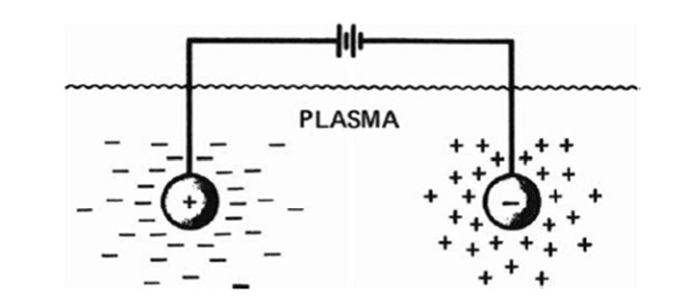
\includegraphics[width=0.7\linewidth]{debye.png}
  \caption{デバイ遮蔽の様子}
  \label{fig.debye}
\end{figure}


雲の中心(荷電粒子の位置)$x=0$のポテンシャルを$\phi _0$として、そこから減少し、無限遠で0になるポテンシャルを考える。このときの$\phi (x)$を求めてみよう。

一次元のポアソン方程式より、

\begin{equation}
  \epsilon_0 \nabla^2 \phi = \epsilon_0 \frac{d^2\phi}{dx^2} = -e(n_i - n_e) \hspace{1pc}  (Z=1) \label{poisson}
\end{equation}
\\
もし遠方の密度が$n_\infty$ であるなら、
\begin{center}
  $n_i = n_\infty$
\end{center}
となる。

ポテンシャルエネルギー$q\phi$の存在下において、電子の分布関数(ボルツマン分布)は、
\begin{equation}
  f(u) = A\exp[-(\frac{1}{2}mv^2 + q\phi)/KT_e]
\end{equation}
$q=-e$として、$u$で積分すると、

\begin{align}
  n_e &= \iiint A\exp[-(\frac{1}{2}mv^2 - e\phi)/KT_e]du^3 = \underline{A}e^{\frac{e\phi}{K T_e}} 
\underset{\equiv n_0}{\underline{\iiint e^{-\frac{m u^2}{2 K T_e}} \, du^3}}\\
       &= n_0 \exp(e\phi/KT_e)
\end{align}
遠方($x\to \infty$)で$\phi \to 0$より、
\begin{center}
  $n_e = n_0\cdot 1 = n_o = n_\infty$
\end{center}
これより、

\begin{center}
 $n_e =  n_\infty \exp(e\phi/KT_e)$
\end{center}
この式は3.5節でより物理的な洞察をもって導く。以上のことから、\eqref{poisson}式を書き直すと、

\[
\epsilon_0 \frac{d^2\phi}{dx^2}= en_\infty(e^{e\phi/KT_e} - 1)
\]
クーロンポテンシャルよりも運動エネルギーの方がはるかに大きい領域、つまり、$|e\phi / KT_e| \ll 1$の領域においてテーラー展開することで、
\[
 \epsilon_0 \frac{d^2\phi}{dx^2} = en_\infty\left[\frac{e\phi}{KT_e}+ \frac{1}{2}(\frac{e\phi}{KT_e})^2 + \cdots \right] \label{telor.1}
\]
さらに、デバイ長を次のように定義する。
\begin{eqbox}{デバイ長}
\begin{equation}
 \lambda_D = \left(\dfrac{\epsilon_0 KT_e}{ne^2}\right)^{1/2} \label{debye}
\end{equation}
\end{eqbox}
これにより、式\refeq{telor.1}の解は、
\begin{equation}
  \phi = \phi_0 \exp(-|x|/\lambda_D) \label{debye.poten}
\end{equation}
となる。デバイ長は遮蔽の距離を決める。密度が増えると$\lambda_D$が減るのは、より電子が集まり、雲が濃くなるからである。$\lambda_D$の定義に使われているのは電子の温度である。なぜなら、電子はイオンに比べはるかに軽く、動きやすいため、電子が動くことにより遮蔽が生じるからである。

式\refeq{debye}の便利な式として、
\begin{align}
  \begin{split}
    \lambda_D &= 69(T_e/n)^{1/2}\si{\metre}, \hspace{2pc}  T_e\, \text{in} \, \si{\kelvin}\\
    \lambda_D &= 7430(KT_e/n)^{1/2}\si{\metre}, \hspace{2pc} KT_e\, \text{in} \, \si{\electronvolt}
  \end{split}
\end{align}
を与えておく。

ここまでで先に述べた「準中性」を定義できる。もし距離$L$の系が$\lambda_D$よりはるかに大きい場合、デバイ遮蔽が生じる。その外では$\nabla^2 \phi$は非常に小さく、$n_i$は$10^{-6}$以上の精度で$n_e$と等しい。
つまり、プラズマの「準中性」とは、$n$をプラズマ密度と呼ばれる一般的な密度とした場合、$n_i \simeq n_e \simeq n$とみなせるほど十分に中性であるが、興味深い電磁気力がすべて消滅するほど中性ではない状態のことである。 

デバイ遮蔽は、電子が非常に高速で互いに衝突せず、熱分布を維持できない場合に破られる。後述するように、電子が非常に高温の場合、電子衝突は稀である。この場合、イオンの正電荷に引き寄せられた一部の電子は、角度をつけて高速で進入し、惑星を周回する衛星のようにイオンの周囲を軌道運動する。
この仕組みは、後述するラングミュアプローブの解説で明らかになる。この効果を「反遮蔽」と呼ぶ者もいる。

1つの種類の系でもデバイ遮蔽は起きることがいえるが、ここでは立ち入らないことにする。

\subsection{プラズマパラメータ}
上で述べたように、デバイ遮蔽が生じるのは「雲」を作るのに十分な粒子が存在するときである。
\refeq{debye.poten}式からデバイ領域の粒子数$N_D$を計算できる。
\begin{equation}
  N_D = n\cdot \frac{4}{3}\pi \lambda_D ^3 = 1.38 \time 10^6T^{3/2}/n^{1/2} \hspace{1pc}(T\text{in}\, \si{\kelvin})
\end{equation}

「集団運動」をするためには、$\lambda_D \ll L$ に加えて、
\begin{equation}
  N_D \lll 1
\end{equation}
が必要である。この$N_D$を\textcolor{red}{プラズマパラメータ}と呼ぶ。

\subsection{プラズマの条件}
イオン化された気体がプラズマとみなされる条件は次の3つである。
\begin{enumerate}
  \item $\lambda_D \ll L$
  \item $N_D \ggg 1$
  \item $\omega \tau > 1$
\end{enumerate}
1,2の条件はこれまでに述べた。3について、プラズマ中の荷電粒子は、電磁力によって支配されている必要がある。
しかし、弱電離ガス(例:飛行機のジェット排気)では、中性粒子との衝突頻度が高すぎるため、運動は流体力学的な力に支配される。
典型的なプラズマ振動の角振動数を$\omega$、中性粒子との平均衝突時間を$\tau$とすると、プラズマと言えるためには、$\omega \tau > 1$が必要である。

\section{1粒子の運動}
\subsection{一様な電場と磁場}
プラズマの解析の難しい点は、流体のように個々の運動は考慮せず、集団運動で考える時もあれば、個々の粒子の集まりと考える時もあることである。
まずは簡単な例として、この章では、1粒子が電場または磁場においての運動を確認しよう。

\subsubsection{E=0}
この系では粒子は単にサイクロトロン運動をする。運動方程式は、
\begin{equation}
  m\frac{d\bm{v}}{dt} = q\bm{v}\times \bm{B} \label{E=0}
\end{equation}
ここで、\bm{B}はz方向を向き、$\bm{B}=B\bm{\hat{z}}$である。\eqref{E=0}式から、
\begin{equation}
\begin{gathered}
  m\dot{v}_x = qB v_y, \quad
  m\dot{v}_y = -qB v_x, \quad
  m\dot{v}_z = 0 \\
  \begin{aligned}
    \ddot{v}_x &= \frac{qB}{m}\dot{v}_y = -\left(\frac{qB}{m}\right)^2 v_x \\
    \ddot{v}_y &= -\frac{qB}{m}\dot{v}_x = -\left(\frac{qB}{m}\right)^2 v_y
  \end{aligned}
\end{gathered}
\end{equation}


  

















\section{結論}
LaTeXを使えば、美しい日本語の文書を作成することができます。ぜひ活用してみてください。




\begin{thebibliography}{99}
\bibitem{a} Francis F. Chen, Introduction to Plasma Physics and Controlled Fusion, Springer; Softcover reprint of the original 3rd ed., 2019\par
\url{http://library.unisel.edu.my/equip-unisel/custom/ebook_catalog/2016BookIntroductionToPlasmaPhysicsAndcompressed.pdf}
\bibitem{b} 宮本健郎, プラズマ物理の基礎, 朝倉書店 , 2014\par
\url{https://op.lib.kobe-u.ac.jp/opac/opac_details/?reqCode=fromlist&lang=0&amode=11&bibid=2002133568&opkey=B175679900718865&start=1&totalnum=4&listnum=1&place=&list_disp=20&list_sort=0&cmode=0&chk_st=0&check=0000}
\bibitem{c} EMANの物理学\par
\url{https://eman-physics.net/electromag/plasma.html}
\end{thebibliography}





\end{document}